\chapter{Methodology \label{ch:methodology}}
This chapter presents the hard- and software used in the \ac{ADS} as it was prepared for the junior flight of \ac{SETH}. The methodology covers a mixture of work done by senior scientists of the \ac{IEAP} and our own contributions. Most notable external contribution comes from Dr. Stephan Böttcher who did the \ac{PCB} design, wrote the \ac{FPGA} code and soldered the example which was used. 

\begin{figure}[H]
    \centering
    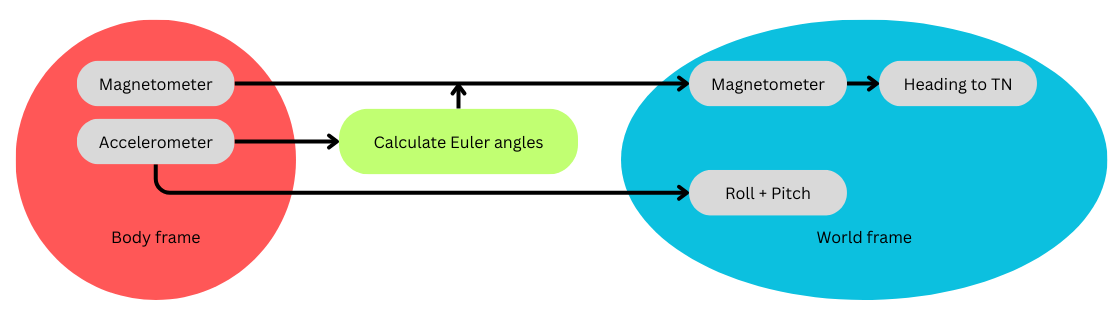
\includegraphics[width=0.75\linewidth]{images/02_methodology/ads_flowchart.png}
    \caption{Flowchart of the methodology.}
    \label{fig:meth:ads_flowchart}
\end{figure}

\section{Data Acquisition \label{sec:meth:data_acquisition}}
The data produced by the accelerometer and magnetometer is stored in \ac{FIFO} buffers until it is requested by the \ac{FPGA}. Once requested the program \verb|rpirena.py| is used to stream the data coming from the \ac{FPGA} to the SD\:Card or the \verb|Asterix| server. This program was written by Dr. Stephan Böttcher and is running on a Raspberry Pi Zero. As of March 14$^\mathrm{th}$ 2025 the program code can be found under \verb|asterix/home/subversion/stephan/solo/eda/cospi/host|. The program writes different event lines into a file, depending on the header of the packet taken from the \ac{FIFO}. The important lines for this thesis are \verb|ID| lines. These lines contain the information from the accelerometer and magnetometer, each entry separated with a white space. Except for the line identifier, all other values are decimal representations of an unsigned 4-bit hexadecimal number, called a word.

The first entry is the line identifier "ID", followed by the packet header 4805$\equiv$0x12C5. After this, the number of words in the line minus one (the packet header is not counted towards this number) is printed. This number is 132 by design. After this number, the information words from accelerometer and magnetometer begin. The first word is the status register of the magnetometer. This contains information if and which data was overwritten and if new data is available. Words three through five are the data output registers in order X, Y, Z. Word six is the temperature data from the magnetometer. Words seven, eight, nine and ten are accelerometer registers containing information about the auxiliary \acp{ADC}. The next batch of words 11 through 64 are 18 magnetometer vectors, one after the other and each in order X, Y, Z. Word 65 is the FIFO\_SRC register of the accelerometer with information about the data contained in the \ac{FIFO}. Word 66 is the status register. Words 67 through 126 are 21 accelerometer vectors, same order as the magnetometer. One more magnetometer vector is read as the last three words 130, 131 and 132. This is illustrated below:
\begin{lstlisting}
#   0     1    2     3    6     7     11   65    66    67   130
ID  4805  132  STAT  MAG  TEMP  STAT  MAG  FIFO  STAT  ACC  MAG
\end{lstlisting}

Because the \acp{FIFO} are read every two seconds, the last magnetometer and accelerometer vector is the same as the second to last.

\section{Data Interpretation \label{sec:meth:data_interpretation}}
To interpret the data, instances of the \textit{ads} class from the \verb|python| script \verb|att_eval.py| are used. Each instance is an object of a specific \verb|.EI| file. The whole file is read with python's built-in \textit{.lineread()} method. The vectors in between two housekeeping ("H") lines are written into an array with $n\cdot20$ lines and 6 columns where n is an integer equal to the number of "ID" lines between the two "H" lines. The times of the vectors are calculated by setting the time of the first vector as the time in the first "H" line minus 1 second. All following times are in 100\,ms steps until the time in the second "H" line minus 1 second is reached. The start time has to start one second earlier because the time that the vectors are measured and digitalized is one second before the time they are requested by the \ac{FPGA}.

The methods \textit{.plot\_vectors()}, \textit{.plot\_sphere()}, \textit{.plot\_angles()} and \textit{.plot\_heading()} are used to display the specified data. The data plotted is: The components of the accelerometer and magnetometer, converted to mGs and units of $g$, against time, the components in three dimensional space, the calculated pitch and roll angles against time and the calculated pitch and roll angles, as well as the heading, against time.

\section{Sensor Calibration Technique \label{sec:meth:calibration_technique}}
The technique applied to calibrate the magnetometer and accelerometer is presented in \parencite{non-orthonogality}. The calibration relies only on the magnitude of the vector field to be measured. This is due to the insight that the flawless measurements of the sensors plotted in three dimensional space all fall onto the surface of a sphere and the radius of the sphere is simply the magnitude of the vector field to be measured. For the earth's magnetic field, $\vec{B}_H$, this is:
\begin{align}
    \vec{B}_H&=\begin{pmatrix} B_x \\ B_y \\ B_z \end{pmatrix} \label{eq:earth_field} \\
    \iff B_H^2& = B_x^2+B_y^2+B_z^2 
    \label{eq:regular_sphere}
\end{align}

If we assume the measurement of each component of the field to be affected by a scale factor and a linear offset, we get the following three equations. The field to be measured is given as in \eqref{eq:earth_field} and we use the superscript $B$ to denote that these are the coefficients for the measurement of the magnetometer.
\begin{align}
    B_{x,\ \mathrm{meas}} &= \frac{B_x}{\sqrt{a^B}}+x_0^B \\
    B_{y,\ \mathrm{meas}} &= \frac{B_y}{\sqrt{b^B}}+y_0^B \\
    B_{z,\ \mathrm{meas}} &= \frac{B_z}{\sqrt{c^B}}+z_0^B
\end{align}

Solving for $B_{x,y,z}$ in each of the formulae above gives us:
\begin{align}
    B_x&=\sqrt{a^B}(B_{x,\ \mathrm{meas}}-x_0^B) \label{eq:bx} \\
    B_y&=\sqrt{b^B}(B_{y,\ \mathrm{meas}}-y_0^B) \label{eq:by} \\
    B_z&=\sqrt{c^B}(B_{z,\ \mathrm{meas}}-z_0^B) \label{eq:bz}
\end{align}

Plugging eqs. \eqref{eq:bx} to \eqref{eq:bz} into eq. \eqref{eq:regular_sphere} gives us the formula for an ellipsoid shifted off the origin by $x_0^B$, $y_0^B$, and $z_0^B$. The half-axes of the ellipsoid are given by the scale factors.
\begin{equation}
    B_{H}^2=a^B(B_{x,\ \mathrm{meas}}-x_0^B)^2 + b^B(B_{y,\ \mathrm{meas}}-y_0^B)^2 + c^B(B_{z,\ \mathrm{meas}}-z_0^B)^2 
    \label{eq:mag_fit_function}
\end{equation}

 Equation \eqref{eq:mag_fit_function} is used to determine the coefficients $a^B$, $b^B$, $c^B$, $x_0^B$, $y_0^B$ and $z_0^B$ using \verb|gnuplot|'s fit function. The measured vectors are given as input for the right hand side of the equation while the square of the magnitude of the earth's magnetic field in Kiel is used for the left hand side.\\
It is now also apparent, why the scale factors in eqs. \eqref{eq:bx} - \eqref{eq:bz} are chosen as one over the square root: the fit converges faster and more accurately when fitting a linear relationship.

While eq. \eqref{eq:mag_fit_function} has been derived for the earth's magnetic field, the same concept is used in the calibration of the accelerometer. The function used to determine the coefficients is eq. \eqref{eq:acc_fit_function}. Because the data is in units of $g$ the magnitude of the field is 1.
\begin{equation}
    1\overset{!}{=}a^g(g_{x,\ \mathrm{meas}}-x_0^g)^2 + b^g(g_{y,\ \mathrm{meas}}-y_0^g)^2 + c^g(g_{z,\ \mathrm{meas}}-z_0^g)^2
    \label{eq:acc_fit_function}
\end{equation}

After the coefficients $a$, $b$, $c$, $x_0$. $y_0$ and $z_0$ are determined for accelerometer and magnetometer, the measured data set is modified as given in eqs. \eqref{eq:bx} - \eqref{eq:bz} to get the true components without measurement error.

A calibration measurement is done to compare two calibration methods. The first method is to lay the sensor down in an orientation for a time of about 60\,s. A new orientation is chosen very 60\,s after this, laying the sensor on a new face of the housing each time. Once all sides (except for the one with the connector) have faced down once, a second method is tested in the same measurement run. The second method is called a "random tumble" in allusion to a random walk. In this random tumble the sensor is rotated randomly around its centre point at a height of around 1.7\,m. To verify the best calibration method, the following steps are done:
\begin{enumerate}
    \item fit coefficients calculated for method I, method II and both
    \item calibrate data set with each set of coefficients
    \item residuals calculated for each set
    \item mean and standard deviation for each residual calculated
    \item the set with lowest mean residual is chosen
\end{enumerate}
The residuals $\Delta B$ of the magnitude of the magnetic field $B=|\vec{B}|$ are calculated according to the following formula:
\begin{equation}
    \Delta B=\frac{B_{\mathrm{meas}}-B_{\mathrm{H}}}{B_{\mathrm{H}}}
    \label{eq:residuals}
\end{equation}


% OPTIONAL: To interpret these mathematical coefficients in a physical sense, the matrices in eqs. \eqref{eq:bg:g_with_errors} and \eqref{eq:bg:b_with_errors} from sec. \ref{sec:bg:measurement_errors} have to be compared to the numerically found coefficients. This complex relationship is shown below in eqs. \ref{eq:coeff_relation_a} and has been derived in appendix \ref{sec:app:deriv_of_coeff}.

\section{Determination of Pitch, Roll and Heading \label{sec:meth:determination_heading}}
The calibrated dataset is used to determine the gondolas heading. For this the magnetic field vector in the body frame (bf) of reference is translated to a world frame (wf) using the accelerometer measurement. After this translation, the components all lie in the correct planes. The last open variable is the orientation of the x-axis in the world frame which is determined using the magnetometer. The acceleration vector in the world frame is given in \eqref{eq:meth:g_vector}. Note that the magnitude of $\vec{g}$ is 1 because measurements are in units of $g$.
\begin{equation}
    \vec{g}^{\ \mathrm{wf}}=\begin{pmatrix} 0 \\ 0 \\ 1 \end{pmatrix} \label{eq:meth:g_vector}
\end{equation}

If the gondola is deflected by an angle, the measurement of the gravity vector will have non zero $x$ or $y$ components. Pitch or roll of the gondola are determined by calculating the arctangent of the $x$ or $y$ components divided by the $z$ component. Using $x$, the result is the pitch angle (i.e. rotation about the y-axis) and using $y$ the result is the roll angle (i.e. rotation about the x-axis).

To compute the heading spherical coordinates are used to describe the gravity vectors position (compare fig. \ref{fig:meth:spherical_coordinates}). We define the angle between the projected vector in the xy-plane and the x-axis as $\varphi\in[-\pi,\pi]$. The angle between the z-axis and the vector is defined as $\vartheta\in[0,\pi]$. Positive angles are counted counter-clockwise, consistent with the right hand rule.

\begin{figure}[H]
    \centering
    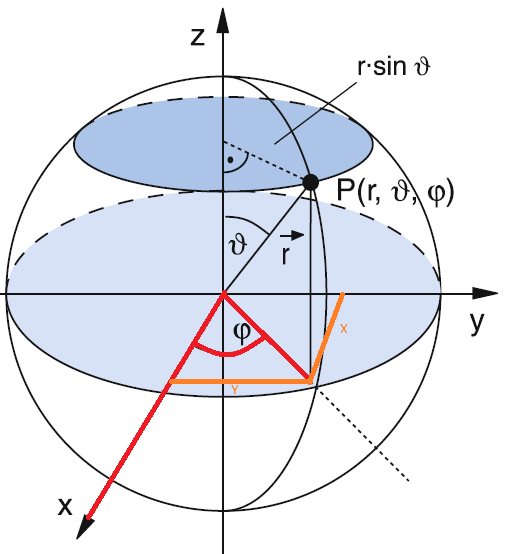
\includegraphics[width=0.5\linewidth]{images/02_methodology/spherical_coords.png}
    \caption[Spherical Coordinates adapted from \parencite{Demtröder2020-mw}.]{Spherical Coordinates in body frame adapted from \parencite{Demtröder2020-mw}. Shown in red is the angle between the projection of the vector $\vec{r}$ and the x-axis. Shown in orange are the $x$ and $y$ components used to calculate pitch and roll.}
    \label{fig:meth:spherical_coordinates}
\end{figure}

To rotate the body frame to the world frame, a rotation of $\varphi$ is performed about the z-axis to align the body frame's x-axis with the deflection of the gravity vector. A second rotation of angle $\vartheta$ about the y-axis aligns the z-axis with the gravity vector. The world frame's xy-plane is now perpendicular to the earth's surface or equivalently: The positive z-axis is now anti-parallel to the normal vector of the earth's surface (i.e. $-\vec{g}$). The heading of the world frame's x-axis is rotated randomly about the z-axis and points in the (random) direction of the gondolas deflection. To determine what heading this is, the measured magnetometer vector is rotated to the world frame as shown below.
\begin{equation}
    \vec{B}_{\mathrm{meas}}^{\ \mathrm{wf}}=R_y(\theta)R_z(\phi)\vec{B}_{\mathrm{meas}}^{\ \mathrm{bf}}
\end{equation}
With the following rotational matrices:
\begin{align}
    R_z(\phi)&=\begin{pmatrix}
                \cos\phi & -\sin\phi & 0 \\
                \sin\phi & \cos\phi & 0 \\
                0 & 0 & 1
                \end{pmatrix} \\
    R_y(\theta)&=\begin{pmatrix}
                \cos\theta & 0 & \sin\theta \\
                0 & 1 & 0 \\
                -\sin\theta & 0 & \cos\theta
                \end{pmatrix}
\end{align}

Seeing as Magnetic North is the direction in which the xy-projection of the magnetic field is pointing, the xy-projection of $\vec{B}_{\mathrm{meas}}^{\ \mathrm{wf}}$ needs to be evaluated. The angle $\psi\in[0,2\pi]$ is the angle between the x-axis of the world frame and the xy-projection of the magnetic field vector (in wf) minus the declination and equivalent to the gondolas heading. The declination $\delta$ of the magnetic field describes the location dependant angle between True and Magnetic North.

By computing pitch, roll and heading as described above, objectives 1 and 2 of this thesis are fulfilled.

Because we use atan2 the -180 to 180 in mathematically positive sense have to mapped to 0 to 360 in math negative sense. 

\section{Reflection on Methodology \label{sec:meth:reflection_methodology}}